\documentclass{article} % For LaTeX2e
\usepackage{iclr2018_conference,times}
\usepackage{hyperref}
\usepackage{url}
\usepackage{graphicx}
%% To use subfigures
\usepackage{subcaption}
%% To place figures where you want to
\usepackage{float}
%% To remove whitespace before enumerate
\usepackage{enumitem}

\title{Deep Sentiment Analysis on Tumblr}

% Authors must not appear in the submitted version. They should be hidden
% as long as the \iclrfinalcopy macro remains commented out below.
% Non-anonymous submissions will be rejected without review.

\author{Anthony Hu \& Seth Flaxman \thanks{ Use footnote for providing further information
about author (webpage, alternative address)---\emph{not} for acknowledging
funding agencies.  Funding acknowledgements go at the end of the paper.} \\
Department of Statistics\\
University of Oxford\\
Oxford, United Kingdom \\
\texttt{\{anthony.hu,flaxman\}@stats.ox.ac.uk} \\
%\And
%Ji Q. Ren \& Yevgeny LeNet \\
%Department of Computational Neuroscience \\
%University of the Witwatersrand \\
%Joburg, South Africa \\
%\texttt{\{robot,net\}@wits.ac.za} \\
%\AND
%Coauthor \\
%Affiliation \\
%Address \\
%\texttt{email}
}

% The \author macro works with any number of authors. There are two commands
% used to separate the names and addresses of multiple authors: \And and \AND.
%
% Using \And between authors leaves it to \LaTeX{} to determine where to break
% the lines. Using \AND forces a linebreak at that point. So, if \LaTeX{}
% puts 3 of 4 authors names on the first line, and the last on the second
% line, try using \AND instead of \And before the third author name.

\newcommand{\fix}{\marginpar{FIX}}
\newcommand{\new}{\marginpar{NEW}}

%\iclrfinalcopy % Uncomment for camera-ready version, but NOT for submission.

\begin{document}


\maketitle

\begin{abstract}
We propose a novel approach to Sentiment Analysis using Deep Neural Networks combining Visual Recognition and Natural Language Processing. Our approach leverages Tumblr posts containing images and text to predict the emotional state of users. Deep convolutional layers extract relevant features from images and high-dimensional word embedding followed by a recurrent layer process the textual information in order to infer the emotion conveyed by a given Tumblr post. We demonstrate that our network architecture, named Deep Sentiment, learns meaningful relations between visual data and language as it vastly outperforms models using a single modality. We then show that Deep Sentiment can also be adapted to generate images and text representative of an emotion. 
\end{abstract}

\section{Introduction}
Sentiment analysis has been an active area of research in the past few years, especially on the readily available Twitter data, e.g. \citet{Bollen} who investigated the impact of collective mood states on stock market or \cite{Seth-16} who analysed day-of-week population well-being.

Contrary to Twitter, Tumblr posts are not limited to 140 characters, allowing more expressiveness, and are not focused on the textual content but on the visual content. A Tumblr post will almost always be an image with some text accompanying the latter. Pictures have become prevalent on social media and characterising them could enable the understanding of billions of users. 

We propose a novel method to uncover the emotional state of an individual posting on social media. The ground truth emotion will be extracted from the tags, considered as the `self-reported' emotion of the user. Our model incorporates both text and image and we aim to `read' them to be able to understand the emotional content they imply about the user. Concretely, the Deep Sentiment model associates the features learned by the two modalities as follows:

\begin{itemize}
    \item We fine-tune a pre-trained Deep Convolutional Neural Network, named Inception \citep{Szegedy-15}, to our specific task of emotion inferring.
    \item We project the text in a rich high-dimensional space with a word representation learned by Word2Vec \citep{Mikolov-13}. The word vectors then go through a Recurrent Neural Network which preserves the word order and captures the semantics of human language.
    \item A fully-connected layer combines the information in the two modalities and a final softmax output layer gives the probability distribution of the emotional state of the user.
\end{itemize}

We will also see that Deep Sentiment can be rearranged to generate Tumblr posts expressing one of the learned emotion.

\section{Tumblr data}

\subsection{The dataset}
Tumblr is a microblogging service where users post multimedia content with the following attributes: an image, text and tags. The tags are really valuable as they indicate the user's state of mind when writing his post. Ekman popularised the idea that there are six basic emotions [cite Ekman]: happiness, sadness, anger, surprise, fear and disgust. These emotions are said to be {\em basic} as they are hardwired regardless of the species: basic emotions are innate, universal, automatic and induce fast reactions that are linked with a high survival rate. [Might need to rewrite when posts with other emotions are added]

To build our dataset, queries were made through the Tumblr API searching for each of the six emotions appearing in the tags. We considered adjectives as they were more commonly used on Tumblr: \#happy, \#sad, \#angry, \#surprised, \#scared and \#disgusted. The emotion would then become the {\em label} of the post that has visual and textual contents as features. Figure \ref{fig:emotions} shows two posts with their associated emotions:

\begin{figure}[H]
    \begin{subfigure}[t]{.5\textwidth}
        \vskip 0pt %Necessary to align on image and not caption
        \centering
        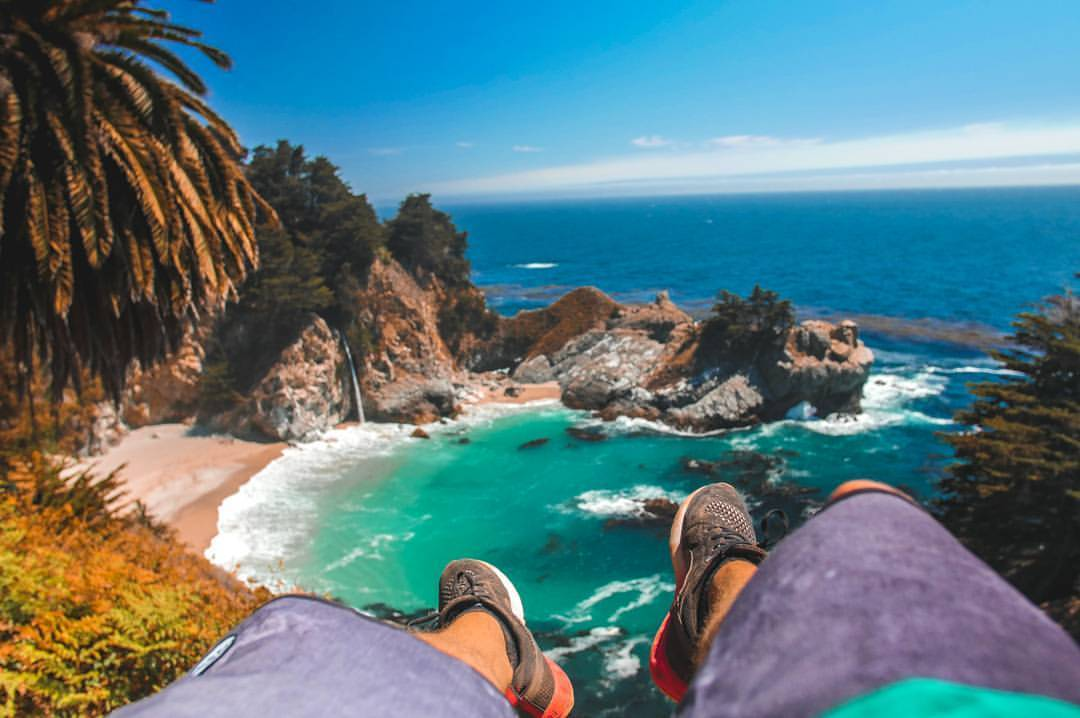
\includegraphics[width=.8\linewidth]{Images/happy.jpg}
        \caption{\textbf{Happy}: ``Just relax with this amazing view \#bigsur \#california \#roadtrip \#usa \#life \#fitness (at McWay Falls)"}
   \end{subfigure}
   \begin{subfigure}[t]{.5\textwidth}
       \vskip 0pt
       \centering
       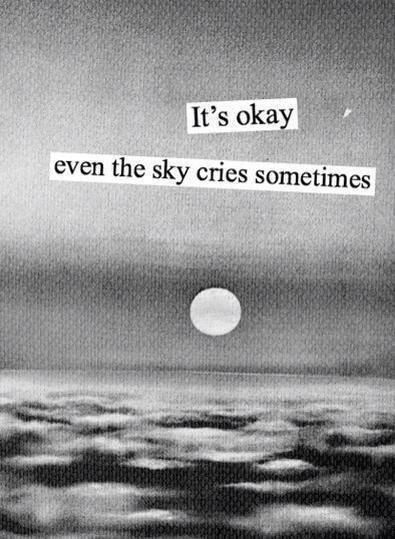
\includegraphics[width=.5\linewidth]{Images/sad.jpg}
       \caption{\textbf{Sad}: ``It's okay to be upset. It's okay to not always be happy. It's okay to cry. Never hide your emotions in fear of upsetting others or of being a bother. If you think no one will listen. Then I will."}
    \end{subfigure}
    \caption{Examples of Tumblr posts}
    \label{fig:emotions}
\end{figure}

\subsection{Data preprocessing}
In some posts, the tag containing the emotion of the post also appeared in the text itself, undermining the possibility of learning meaningful relationships between the features and the emotion expressed. We thus removed from the text the tags containing the emotion to be predicted.

Tumblr is used worldwide but we only kept posts written in English. Basically, if a post contained less than a given number of English word, it was deemed as non-English and removed from the dataset. The threshold was set to 5 English words as it appeared to filter out reasonably well non-English posts. [To change: filter posts with less than 90\% of English words] The vocabulary of English words was obtained from Word2Vec.

[talk about dataset size, and reduction through preprocessing]

\section{Visual recognition}
Pictures are valuable to accurately infer the emotion expressed by a user. For instance, happy photos might contain sunny landscapes while sad pictures might contain darker colors. To extract visual insights from images, we will use convolutional neural networks, which achieve state-of-the-art performances in many visual recognition tasks.

\subsection{Transfer learning}
Training a convolutional network from scratch can be difficult as a large amount of data is needed and many different architectures need to be tested before achieving satisfying performances. To circumvent this issue, we can take advantage of the pre-trained network named Inception [cite] that learned to recognise images through the ImageNet dataset with a deep architecture of 22 layers.

Inception learned representations capturing the colors and arrangement of shapes of an image, which turn out to be relevant when dealing with images even for a different task. We could also say that the pre-trained network grasped the underlying structure of images. This statement rests on the hypothesis that all images are in a low-dimensional manifold, and recent advances in realistic photos generation through generative adversarial networks bolsters this idea [cite Radford, Unsupervised Representation Learning with Deep Convolutional Generative Adversarial Networks.]. 

More specifically, the Inception network learned to recognise features in a picture in order to classify the latter among the 1000 classes in the ImageNet dataset. Suppose that instead of classifying an image into 1000 classes we want to label it according to 6 different emotions (happy, sad, angry, scared, surprised, disgusted). The same features can be combined in a different way to let the network take a decision about what the emotion conveyed by the image is.

The process described above is called {\em Transfer Learning}: we chop off the last layer of the network and add our own layer given how many classes we have. We then freeze the weights of the other layers and only backpropagate through the newly created layer when training the network on our examples. If we have enough data, we can unfreeze more higher-level layers and backpropagate through them.

\subsection{Results}
The Inception model was fed raw images, that were resized to a fixed size $(224, 224, 3)$, and fine-tuned with the following parameters:
\begin{itemize}[topsep=0pt]
    \item 9,000 training steps
    \item Mini-batch of size 32
    \item Adam optimizer with a learning rate of $1\mathrm{e}{-6}$
\end{itemize}

After the preprocessing described in Section 2, the dataset contains 295,508 posts that we split as 80\% train set and 20\% test set. The metric used to evaluate the model is accuracy, which is the fraction of correctly classified images.

The fine-tuned Inception is compared to a baseline: random guessing that includes the prior probabilities of the classes: 
\begin{table}[H]
\caption{Prior probabilities of the classes}
\begin{center}
    \begin{tabular}{| c | c | c | c | c | c | c |}
    \hline
     & \textbf{happiness} & \textbf{sadness} &  \textbf{anger} & \textbf{surprise} & \textbf{fear} & \textbf{disgust} \\ \hline
    \textbf{Prior proba.} & 0.32 & 0.22 & 0.19 & 0.03 & 0.22 & 0.02 \\
    \hline
    \end{tabular}
\end{center} 
\end{table}

The results are:
\begin{table}[H]
\caption{Image model against random guessing}
\begin{center}
    \begin{tabular}{| l | c | c |}
    \hline
    & \textbf{Train} & \textbf{Test} \\
    & \textbf{accuracy} & \textbf{accuracy} \\ \hline
    \textbf{Random guessing} & 24\% & 24\% \\ \hline
    \textbf{Inception fine-tuned}  & 48\% & 42\% \\
    \hline
    \end{tabular}
\end{center} 
\end{table}

\section{Natural language processing}
Even as a human being, it can be difficult to guess the expressed emotion by only looking at a Tumblr image without reading its caption as shown by Figure \ref{surprised-unclear}.

\begin{figure}[H]
    \centering
    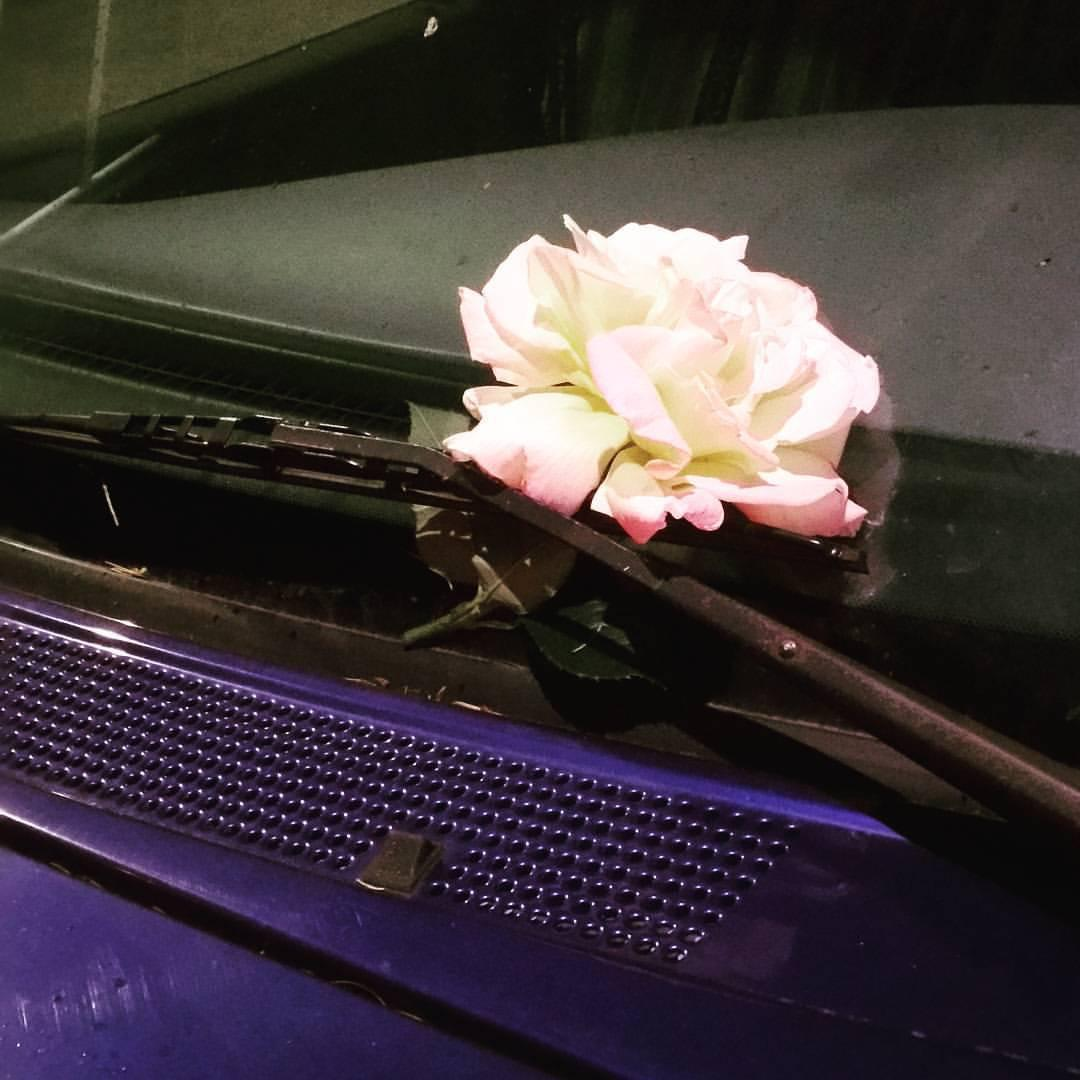
\includegraphics[width=0.3\textwidth]{Images/flower.jpg}
    \caption{Which emotion is it?}
    \label{surprised-unclear}
\end{figure}

It's unclear whether the user wants to convey happiness or surprise. Only by reading the text ``To who ever left this on my windshield outside of last nights art opening, I love you. You made my night.", we can finally conclude that the person was {\em surprised}. The text is extremely informative and is usually crucial to accurately infer the expressed emotion.

\subsection{Word embedding}

Neural networks only accept numbers as inputs, therefore the text has to be converted beforehand. A very successful way to capture the meaning of textual information is by using word embedding. Most learning algorithms rely on the local smoothness hypothesis, that is, similar training instances are spatially close. This hypothesis clearly doesn't hold with one-hot encoding as `dog' is as close to `tree' as it is to `cat'. Ideally, we would like to transform the word `dog' in a space so that it's closer to `cat' than it is to `tree'. That's exactly how word embedding works: every word is projected into a high-dimensional space that preserves semantic relationships. Therefore, what the model has learned about dogs can be used when faced with a cat.

We will be using Word2Vec [elaborate]

Each post in the dataset does not necessarily contain the same number of words. Even after embedding each word, the input will be of variable size and most learning algorithm expect a fixed-sized input. To solve that problem, we can simply average across the number of words. The information loss is still minimal as the features come from a high-dimensional space [cite seth1]

However note that the word order is completely lost. Human language relies on the word order to communicate as for example the word {\em change} can be both a noun and a verb, and negation such as `not entertained' can only be understood if `not' directly precedes the verb.

The order information can be preserved using Recurrent Neural Networks

\subsection{RNN}
Each post will be broken down into a sequence of words and then fed to an LSTM [cite] that will infer the emotion of the user. On a more technical note, the vector of words will be represented by a list of ids from the Word2Vec vocabulary say $[3, 20, 1, 49, 6]$. To account for shorter posts, we'll have to zero-pad the vector -- the id 0 will actually be associated with a word token $<$PAD$>$ -- like $[3, 20, 1, 49, 6, 0, 0, ..., 0]$. For longer posts, we'll only keep the 200 first words. The model is:
\begin{itemize}
    \item Word embedding into a vector of dimension 300.
    \item An LSTM layer of size 512.
    \item An output layer of size 6.
\end{itemize}

\subsection{Result}
The network was trained with:
\begin{itemize}[topsep=0pt]
    \item 10,000 training steps
    \item Mini-batch of size 128
    \item Adam optimizer with an initial learning rate of 0.01
    \item Learning rate decay of $\frac{1}{2}$ every 1000 steps
    \item LSTM unrolled for 20 words
    \item Gradient clipping with a maximum norm of 5.0
\end{itemize}

\begin{table}[H]
\caption{Text model against random guessing}
\begin{center}
    \begin{tabular}{| l | c | c |}
    \hline
    & \textbf{Train} & \textbf{Test} \\
    & \textbf{accuracy} & \textbf{accuracy} \\ \hline
    \textbf{Random guessing} & 24\% & 24\% \\ \hline
    \textbf{LSTM}  & 63\% & 61\% \\
    \hline
    \end{tabular}
\end{center} 
\end{table}


\section{Citations, figures, tables, references}
\label{others}

These instructions apply to everyone, regardless of the formatter being used.

\subsection{Citations within the text}

Citations within the text should be based on the \texttt{natbib} package
and include the authors' last names and year (with the ``et~al.'' construct
for more than two authors). When the authors or the publication are
included in the sentence, the citation should not be in parenthesis (as
in ``See \citet{Hinton06} for more information.''). Otherwise, the citation
should be in parenthesis (as in ``Deep learning shows promise to make progress towards AI~\citep{Bengio+chapter2007}.'').

The corresponding references are to be listed in alphabetical order of
authors, in the \textsc{References} section. As to the format of the
references themselves, any style is acceptable as long as it is used
consistently.

\subsection{Footnotes}

Indicate footnotes with a number\footnote{Sample of the first footnote} in the
text. Place the footnotes at the bottom of the page on which they appear.
Precede the footnote with a horizontal rule of 2~inches
(12~picas).\footnote{Sample of the second footnote}

\subsection{Figures}

All artwork must be neat, clean, and legible. Lines should be dark
enough for purposes of reproduction; art work should not be
hand-drawn. The figure number and caption always appear after the
figure. Place one line space before the figure caption, and one line
space after the figure. The figure caption is lower case (except for
first word and proper nouns); figures are numbered consecutively.

Make sure the figure caption does not get separated from the figure.
Leave sufficient space to avoid splitting the figure and figure caption.

You may use color figures.
However, it is best for the
figure captions and the paper body to make sense if the paper is printed
either in black/white or in color.
\begin{figure}[h]
\begin{center}
%\framebox[4.0in]{$\;$}
\fbox{\rule[-.5cm]{0cm}{4cm} \rule[-.5cm]{4cm}{0cm}}
\end{center}
\caption{Sample figure caption.}
\end{figure}

\subsection{Tables}

All tables must be centered, neat, clean and legible. Do not use hand-drawn
tables. The table number and title always appear before the table. See
Table~\ref{sample-table}.

Place one line space before the table title, one line space after the table
title, and one line space after the table. The table title must be lower case
(except for first word and proper nouns); tables are numbered consecutively.

\begin{table}[t]
\caption{Sample table title}
\label{sample-table}
\begin{center}
\begin{tabular}{ll}
\multicolumn{1}{c}{\bf PART}  &\multicolumn{1}{c}{\bf DESCRIPTION}
\\ \hline \\
Dendrite         &Input terminal \\
Axon             &Output terminal \\
Soma             &Cell body (contains cell nucleus) \\
\end{tabular}
\end{center}
\end{table}

\subsubsection*{Acknowledgments}

Use unnumbered third level headings for the acknowledgments. All
acknowledgments, including those to funding agencies, go at the end of the paper.

\bibliography{iclr2018_conference}
\bibliographystyle{iclr2018_conference}

\end{document}
